%%%%%%%%%%%%%%%%%%%%%%%%%%%%%%%%%%%%%%%%%%%%%%%%%%%%%%%%%%%%%%%%%%%%%%%%%%%%%%%%
% Author : Hai Phong Nguyen, Tomas Polasek (template)
% Description : Seventh exercise in the Introduction to Game Development course.
%   It deals with the creation of a Game Design Document, presenting a short 
%   pitch for a potential game project.
%%%%%%%%%%%%%%%%%%%%%%%%%%%%%%%%%%%%%%%%%%%%%%%%%%%%%%%%%%%%%%%%%%%%%%%%%%%%%%%%

\documentclass[a4paper,10pt,english]{article}

\usepackage[left=2.50cm,right=2.50cm,top=1.50cm,bottom=2.50cm]{geometry}
\usepackage[utf8]{inputenc}

% Hyper-Text References
\usepackage{hyperref}
\hypersetup{colorlinks=true, urlcolor=blue}

% Drawing Images and Graphs
\usepackage{tikz}
\usepackage{pgfplots}

% Page Utilities
\usepackage{graphicx}
\graphicspath{ {.} }

% Image Sub-Captions
\usepackage{subcaption}

\newcommand{\ph}[1]{\textit{[#1]}}

\title{%
Game Pitch Document%
}
\author{%
Hai Phong Nguyen (xnguye28)%
}
\date{31.12.2023}

\begin{document}

\maketitle
\thispagestyle{empty}

{%
\large

\begin{itemize}

\item[] \textbf{Title:} \ph{Lost worlds}

\item[] \textbf{Genre:} \ph{Story-based adventure with survival elements}

\item[] \textbf{Style:} \ph{Pixel-art stylized 3D}

\item[] \textbf{Platform:} \ph{PC, PlayStation consoles, XBox consoles}

\item[] \textbf{Market:} \ph{Singleplayer games, open-world games}

\item[] \textbf{Elevator Pitch:} \ph{A story-based game with a rich world that lives on its own)}

\end{itemize}

}

\section*{\centering The Pitch}

\subsection*{Introduction}
The Lost Worlds is a visual story-telling adventure game. The main goal is to build an immersive world, full of stories and life. Players will have to uncover the origins of the world they are put into, while trying to survive and adapt to their surroundings.
\subsection*{Background}
The inspiration is drawn from various sources, mostly games and animations. The goal of telling a visual story, while still keeping the challenging and stimulative aspect of the game should be a blend between classical gaming and filmography. Main inspirations for the game mechanics come from the game "Rain World", in which the self-sustained ecosystem plays a big role. The visual appearance is heavily inspired by an indie game developer t3ssel8r's work.

\subsection*{Setting}
The game is set in an alternative world, perhaps on another planet. The main playable character is a lonely wandering creature, desperately searching for the rest of his kind. The abandoned ruins and remnants of man-made structures reveal, that the player may be one of the last surviving members of a past civilisation. Perhaps the different events occurring in the game's nature will tell the player more about the possible story of the civilisation's downfall.

The planet is lush in resources, and various animals and plants inhabit it. Some are shy and hard to find, others may be hostile. Our main character is also a part of the ecosystem, meaning that both positive and negative interactions may take place during the adventure. The inter-species interactions will not only be between the main character and the non-playable characters, but also between non playable creatures aswell.

\subsection*{Features}
Following a success of Rain World, our game will offer a breathtaking world that lives on its own. Beside the main story, players will have a chance to discover the inner workings of the ecosystem, observe how different kinds of living and non-living elements interact with each other, creating countless of additional stories. We aim to differentiate from other story-based games by allowing players to dictate the flow of the story.  Our target audience is a group of players wanting to experience a story based game with big replay potential.

\begin{itemize}
    \item The game will simulate realistic behaviour between different kinds of creatures, plants and terrain.
    \item Weather will have a real impact on the world, forcing players to adapt their play-style to certain weather conditions.
    \item The game will offer a variety of goals beside the story, such as domesticating different creatures, finding rare locations with unseen scenery and advanced system of cooking, utilizing resources from specific locations.
    \item The story is driven by the player, there will be no hard-coded objectives
\end{itemize}

\subsection*{Genre}
The Lost Worlds is a story-based, open world adventure with survival elements. The survival elements, derived from the ecosystem of the world, play a big role in understanding the story itself. 

\subsection*{Platform}
The game will be developed for PC. Release for consoles will be planned after beta play-testing.

\subsection*{Style}
The game will be rendered in 3D, using various techniques to achieve a simplistic, yet visually appealing pixelated look.

\vspace{1cm}
\begin{figure}[h]
\centering
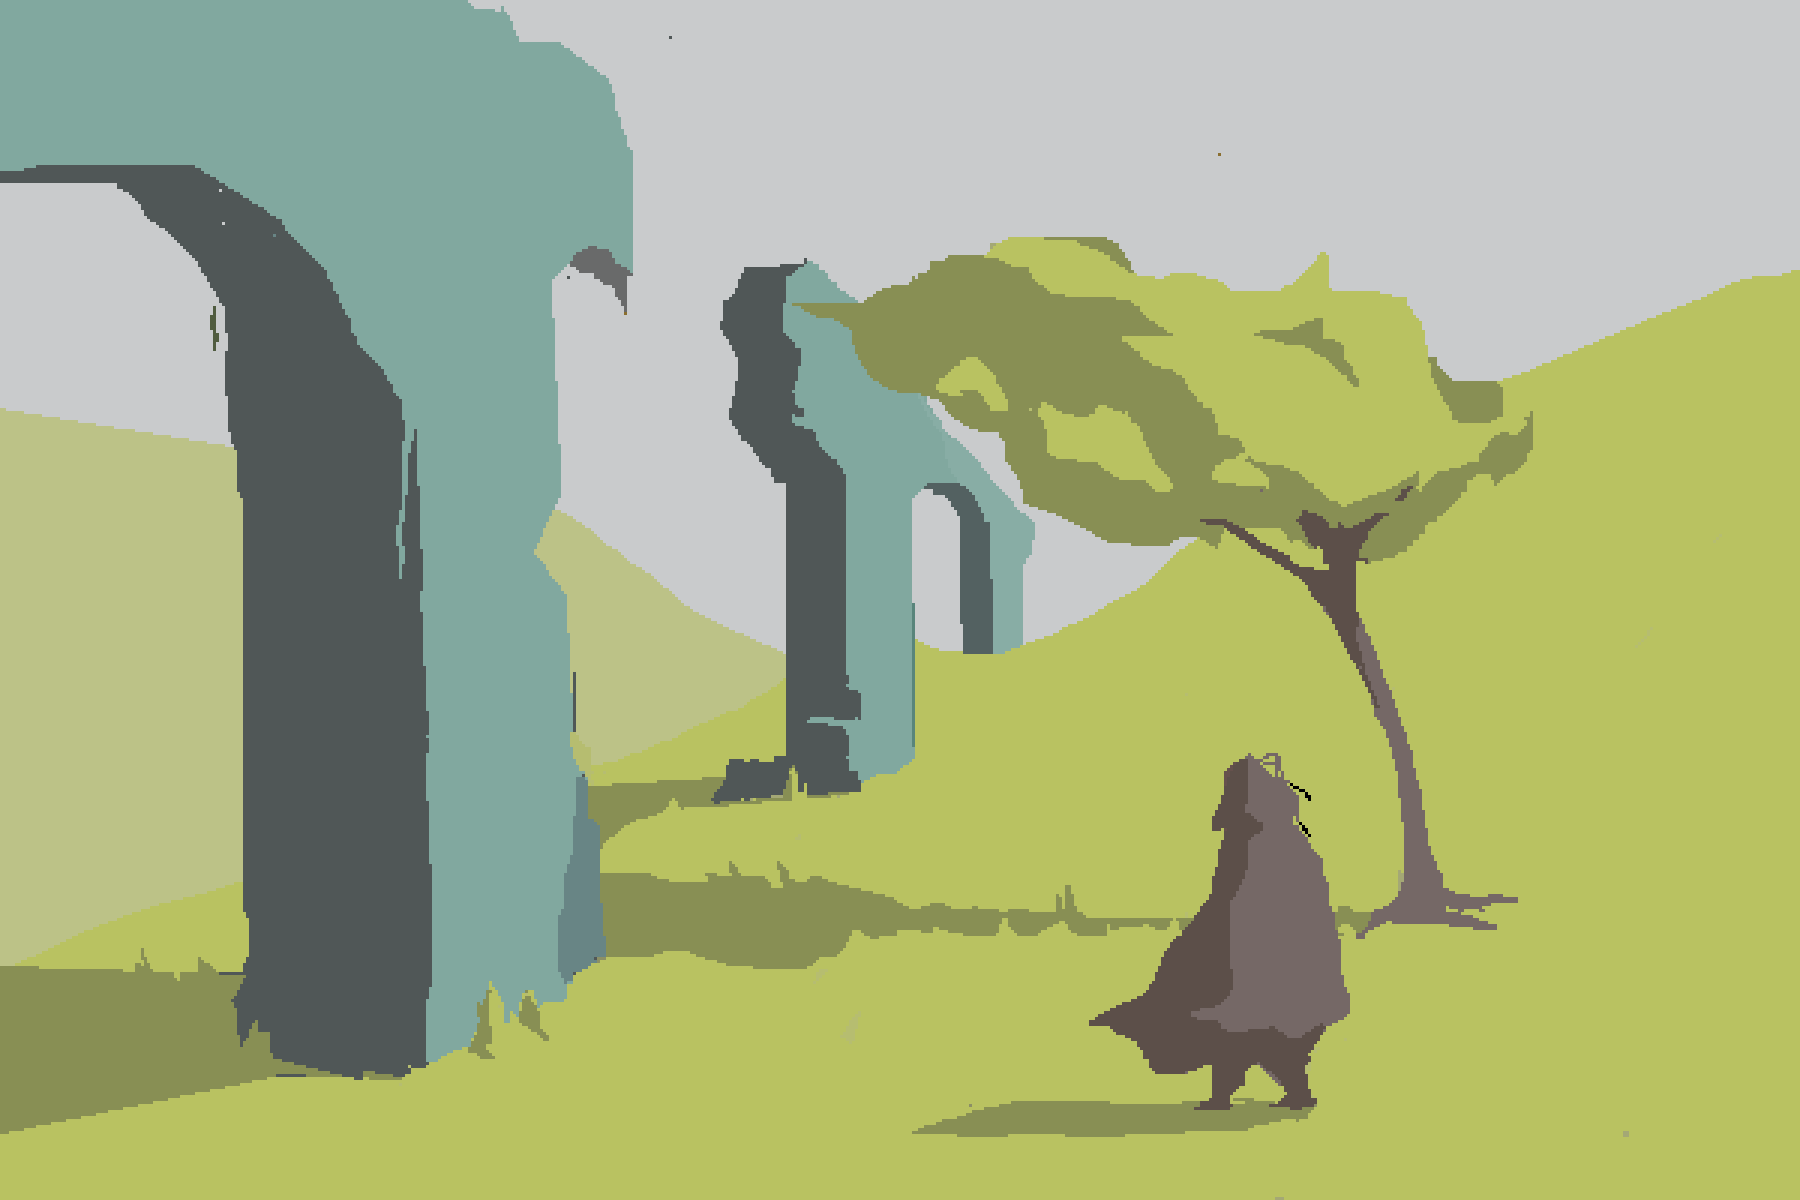
\includegraphics[width=300px,height=\textheight,keepaspectratio]{pitch}
\captionof{figure}{Visual style concept art}
\end{figure}

\end{document}
